A cold gas thruster (CGT) is a system that uses expanding gas to generate a force. This force is typically used in reaction control systems (RCSs) to stabilize space craft or simply change their attitude. This paper is primarily concerned with reaction control systems to be developed for high altitude balloon payloads (HABPs.) These HABPs experience intense and sporadic winds. Winds which make data collection for certain sensors difficult. There are several ways in which a RCS can achieve stabilization, but the method of choice here is the CGT.\\
There are several components important to the CGT RCS. Here, there will only be a brief discussion on two of these components such that the analysis is not lacking information. \\
The first consideration to make is the type of gas to be used. The primary question here is, \textit{what makes one gas better than another?} One parameter that tries to answer this question is the \textit{specific impulse} ($I_{sp}$). This is a value specific to a gas. Experimentally, it is measured by integrating a force (F) versus time (t) plot generated by a CGT using that gas. That will give the total impulse, this is divided by the change in weight of the gas through that time period ($\tau$). In other words:
\begin{equation}\label{eq:ExperimentalIsp}
I_{sp}=\frac{\sum\limits_{t=0}^{\tau} F(t)t}{\Delta mg}
\end{equation}%
\nomenclature{$I_{sp}$}{Specific impulse}%
\nomenclature{$t$}{Time}%
\nomenclature{$m$}{Mass}%
\nomenclature{$g$}{Acceleration due to gravity}%
\nomenclature{$F$}{Force or thrust}%
where $\Delta m$ is mass and g is acceleration due to gravity. More precisely, specific impulse is defined by  equation \ref{eq:DefineSpecificImpulse}.
\begin{equation}\label{eq:DefineSpecificImpulse}
I_{sp}=\frac{F}{dm/dt}
\end{equation}
You may notice the descrepency in units between equations \ref{eq:ExperimentalIsp} and \ref{eq:DefineSpecificImpulse}. Often times the $I_{sp}$ is given with units of s, but in reality it is defined with units of $Ns/kg$.\\
This is an excellent start to creating a standard for comparing gases, but there is much more that should be considered. Factors such as safety, availability, cost, energy storage density, and so on all contribute to the choice of gas. Additionally, each one of these factors has a different weight per say depending on the scenario in which they are being applied. After consideration, the choice of gas for this system is $CO_2$.\\
The other component is the nozzle. These are used to set the mass flow rate for the system and to accelerate the propellant to supersonic speeds. They consist of a converging section that leads into a throat of minimum radius and a diverging section. Figure \ref{fig:Nozzle} shows a simple 2D section of a typical nozzle. 
\begin{figure}[h!]
\centering
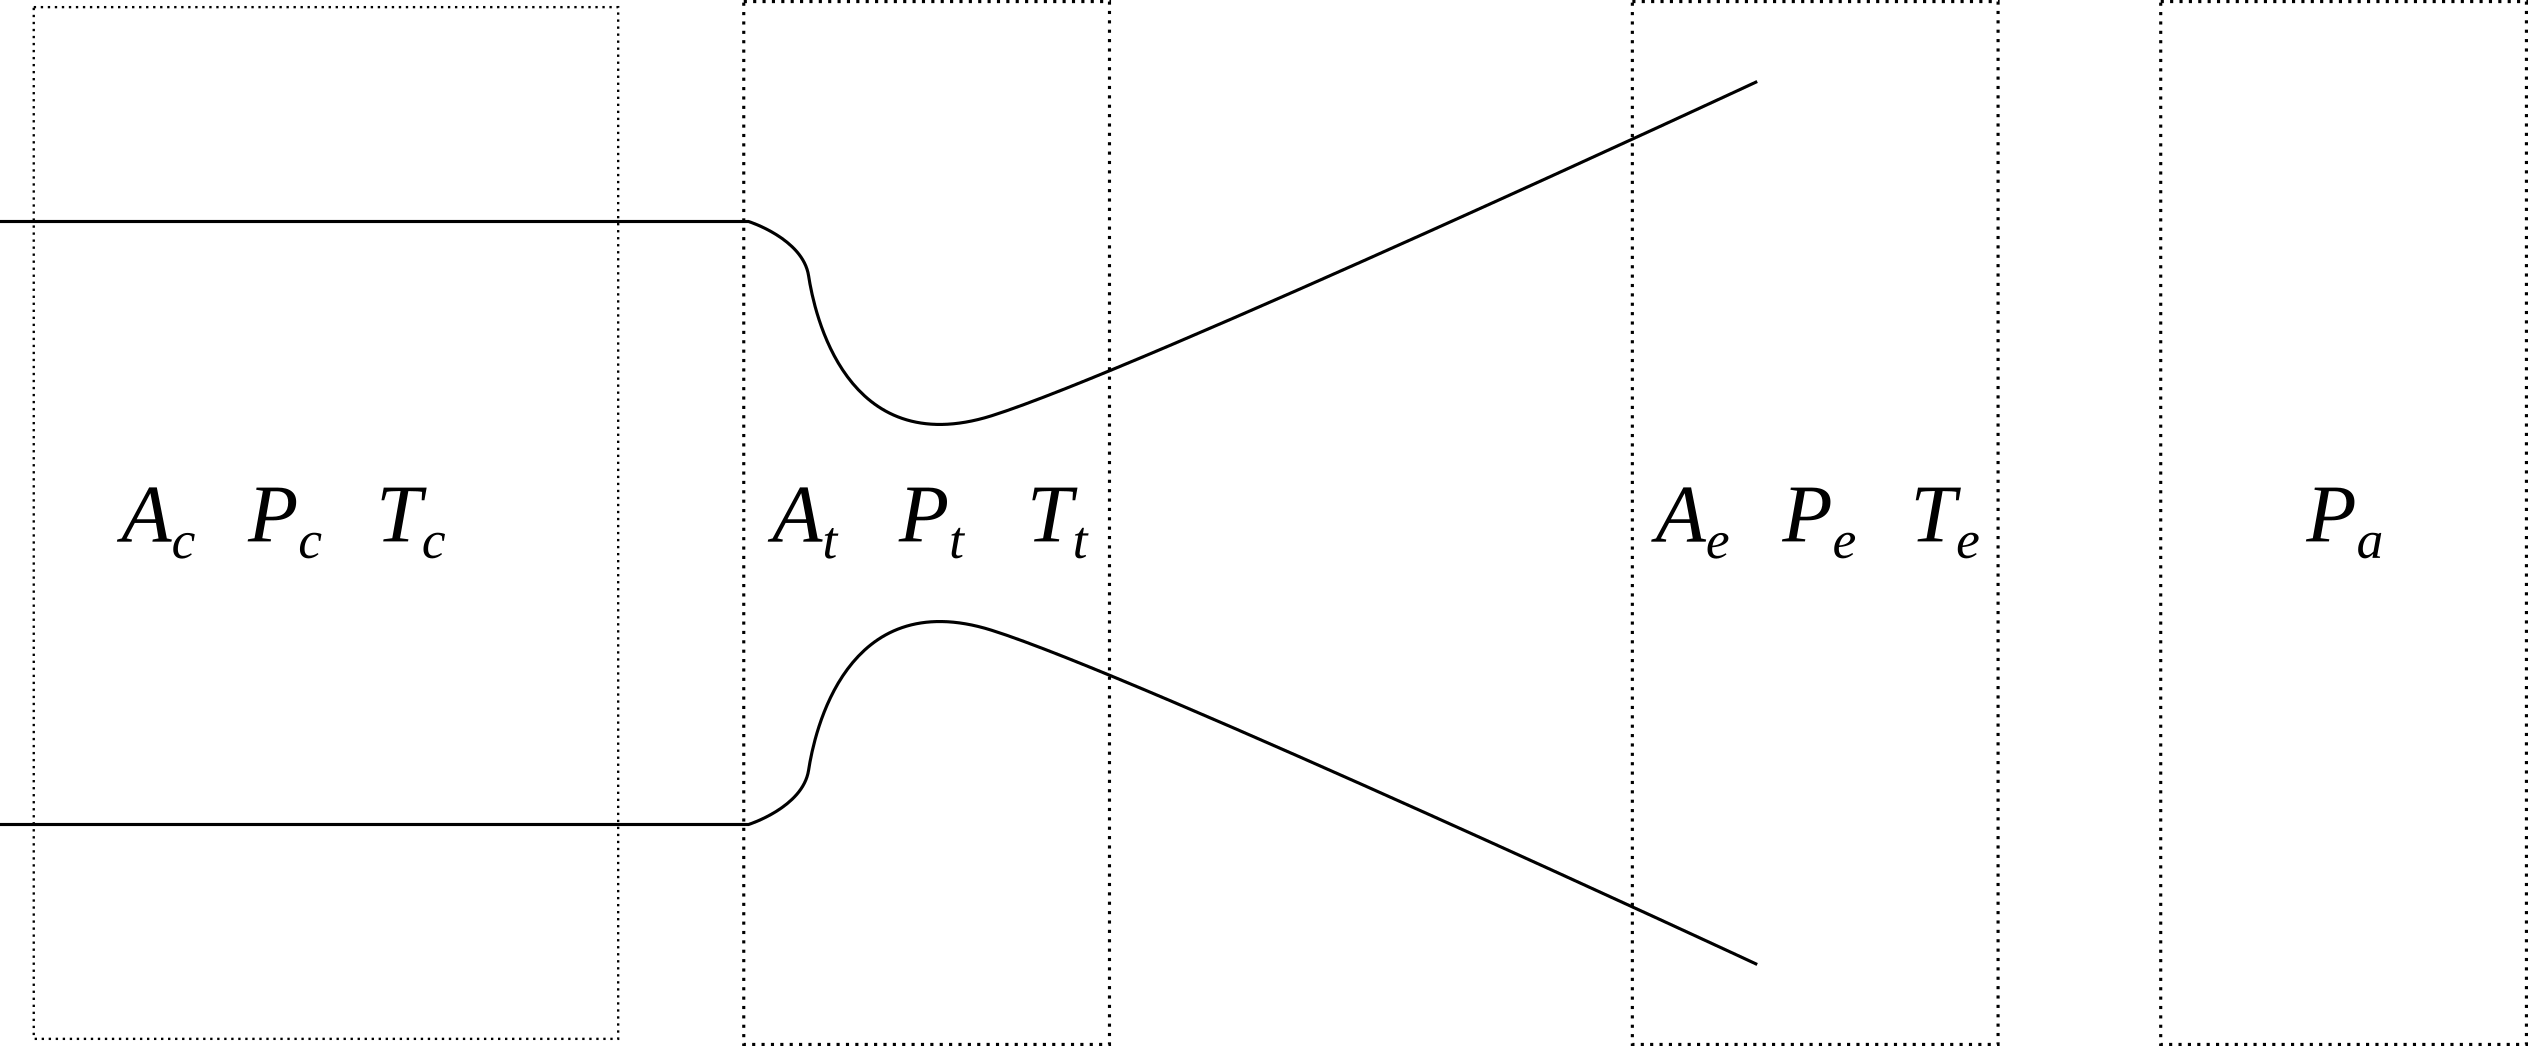
\includegraphics[scale=.5]{Figures/DefineNozzle}
\caption{Simple nozzle cross-section showing four regions of interest}
\label{fig:Nozzle}
\end{figure}
The four regions of this nozzle are the chamber (c), throat (t), exit (e), and ambient (a). Some variables of interest are shown for each region.\\
Nozzles that have been made to achieve maximum thrust obey the following characteristics. In the converging section, the gas is accelerated; once the throat is reached the gas is traveling at the speed of sound. Then, as it proceeds into the diverging section, it continues to accelerate until it reaches the exit plane of the nozzle. Ideally, the nozzle is designed such that the pressure of the gas exiting the nozzle is equal to the ambient pressure. \\
The thrust produced by a nozzle can be written in terms of the variables listed below. First, though, it is given by equation \ref{eq:1.64} in reference \cite{RocketPropulsion}.
\begin{itemize}
\item Chamber Temperature ($T_c$)
\item Exit Temperature ($T_e$)
\item Chamber Pressure ($P_c$)
\item Exit Area of Nozzle ($A_e$)
\item Throat Area of Nozzle ($A_t$)
\end{itemize}%
\nomenclature{$P_c$}{Chamber pressure}%
\nomenclature{$T_e$}{Exit temperature}%
\nomenclature{$T_c$}{Chamber temperature}%
\nomenclature{$A_e$}{Exit area of nozzle}%
\nomenclature{$A_t$}{Throat area of nozzle}%
The derivation will not be shown here, but reference \cite{RocketPropulsion} discusses it in detail. The text derives equation \ref{eq:1.64} from the laws of thermodynamics and some general assumptions.
\begin{equation}\label{eq:1.64}
C_F= \sqrt{\frac{2\gamma^2}{\gamma-1}\left(\frac{2}{\gamma+1}\right)^{\frac{\gamma+1}{\gamma-1}}\left(1-\left(\frac{P_e}{P_c}\right)^{\frac{\gamma-1}{\gamma}}\right)}+\frac{\left(P_e-P_a\right)}{P_c}\frac{A_e}{A_t}
\end{equation}%
\nomenclature{$C_F$}{Thrust coefficient}%
\nomenclature{$P_a$}{Ambient pressure}%
\nomenclature{$P_e$}{Exit pressure}%
\nomenclature{$\gamma$}{Ratio of specific heats}%
Where $C_F$ is defined by:
\begin{equation}\label{eq:ThrustCoefficient}
C_F=\frac{F}{A_tP_c}
\end{equation}
It is also helpful to define the nozzle's expansion ratio ($\epsilon$), given by equation \ref{eq:ExpansionRatio}.
\begin{equation}\label{eq:ExpansionRatio}
\epsilon=\frac{A_e}{A_t}
\end{equation}%
\nomenclature{$\epsilon$}{Area expansion ratio for nozzle}
It can be seen $C_F$, ergo the thrust, is at maximum when $P_a=P_e=0$. It is also shown that $\frac{P_e}{P_c}$ is given by equation \ref{eq:PressureRatio}.
\begin{equation}\label{eq:PressureRatio}
\frac{P_e}{P_c}=\left(1+\frac{(\gamma-1)}{2}M^2\right)^{\frac{\gamma}{\gamma-1}}
\end{equation}%
\nomenclature{$M$}{Mach number}%
Additionally, we can define the mach number as:
\begin{equation}\label{eq:MachNumber}
M^2=\frac{2}{\gamma-1}\left(\frac{T_c}{T_e}-1\right)
\end{equation}
allowing us to make a substitution for $\frac{P_e}{P_c}$ into equation \ref{eq:1.64}. With this substitution, we will eliminate $P_e$. The motivation for this is that measuring the exit plane pressure is more difficult than measuring the exit plane temperature. After the subtitutions, we retrieve equation \ref{eq:NozzleForce}.
\begin{equation}\label{eq:NozzleForce}
F = A_t P_c \left(\sqrt{\frac{2\gamma^2}{\gamma-1}\left(\frac{2}{\gamma+1}\right)^{\frac{\gamma+1}{\gamma-1}}\left(1-\frac{T_e}{T_c}\right)}+\left(\left(\frac{T_e}{T_c}\right)^{\frac{\gamma}{\gamma-1}}-\frac{P_a}{P_c}\right)\epsilon\right)
\end{equation}
This equation was developed given some assumptions and in different systems some of the assumptions may have a more or less dominant effect. It can also be seen that since the thrust is highly dependent on the external pressure, the nozzle should be designed to maximize the thrust in the pressure it will spend the most time in. Because of this an experiment was developed to determine the reliability of equation \ref{eq:NozzleForce}.\\
In measuring the thrust at several different area ratios and comparing it to the predicted thrust, the hope is to create an "effective" proportionality constant. This would then allow the nozzle design process to be maximized for pressures that cannot be tested on Earth's surface.
